% Name: Regular hexagon and its apothem
% Description: A regular hexagon with side s, circumradius r = s, and apothem a = (√3/2)s at 30° to the radius, so its area is half the perimeter times the apothem.
% Tags: regular polygon, apothem, hexagon, area

\usetikzlibrary{angles, quotes}

\begin{tikzpicture}[thick, every node/.style={font=\small}]
  \coordinate (O) at (0,0);
  \coordinate (P) at (-30:2.5);
  \coordinate (Q) at (30:2.5);
  \coordinate (M) at (0:{2.5*cos(30)});
  \draw[fill=blue!8] (-30:2.5) \foreach \k in {1,...,5} { -- (-30+60*\k:2.5) } -- cycle;
  \fill[orange!20] (O) -- (P) -- (Q) -- cycle;
  \draw[orange!85!black] (O) -- node[below left] {$r$} (P) (O) -- (Q);
  \draw[very thick, orange!85!black] (P) -- node[right] {$s$} (Q);
  \draw[blue!70!black] (O) -- node[below, pos=0.6] {$a$} (M);
  \pic[draw, thin, angle radius=2mm] {right angle=O--M--Q};
  \pic[draw, thin, angle radius=7mm, "$30^\circ$", angle eccentricity=1.6] {angle=M--O--Q};
  \fill (O) circle (1.5pt) node[left] {$O$};
  \node[anchor=west] at (3.1,0.4) {$a = \tfrac{\sqrt{3}}{2}\,s$};
  \node[anchor=west] at (3.1,-0.4) {$A = \tfrac{1}{2} \cdot 6s \cdot a$};
\end{tikzpicture}
